%Como se juntan las definiciones con lo demas
\section{Conjuntos de prueba}
Existesn 

\section{Metaheurísticas aplicadas al JSP}
Las metaheurísticas han conseguido hallar buenas soluciones para los conjuntos de prueba 
% ve como se pueden mejorar 
U

% poblacionales 



\subsection*{Vecindades previamente propuestas}
Se han propuesto varias estructuras de vecindad al JSP, a continuación se describen las más importantes a la fecha:

\begin{itemize}
\item N1 \cite{blazewicz1996job} Consiste en considerar todas las soluciones que se crean al intercambiar cualquier par de operaciones adyacentes que pertenecen a un bloque crítico. Esta vecindad es muy grande y considera muchos cambios que no mejoran el makespan.
\begin{figure}[H]
\centering
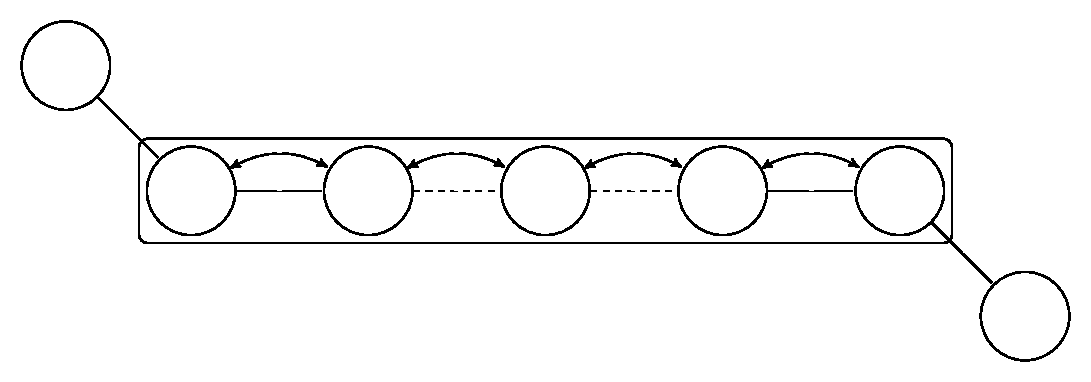
\includegraphics[scale=.7]{Imagenes/N1.pdf}
\caption{Movimientos de la vecindad N1}
\end{figure}

\item N4 \cite{dell1993applying} Esta vecindad se propuso como un refinamiento y extensión de la vecindad N1 y toma como base el concepto de bloque crítico. Consiste en llevar operaciones internas del bloque crítico al inicio o final. 
\begin{figure}[H]
\centering
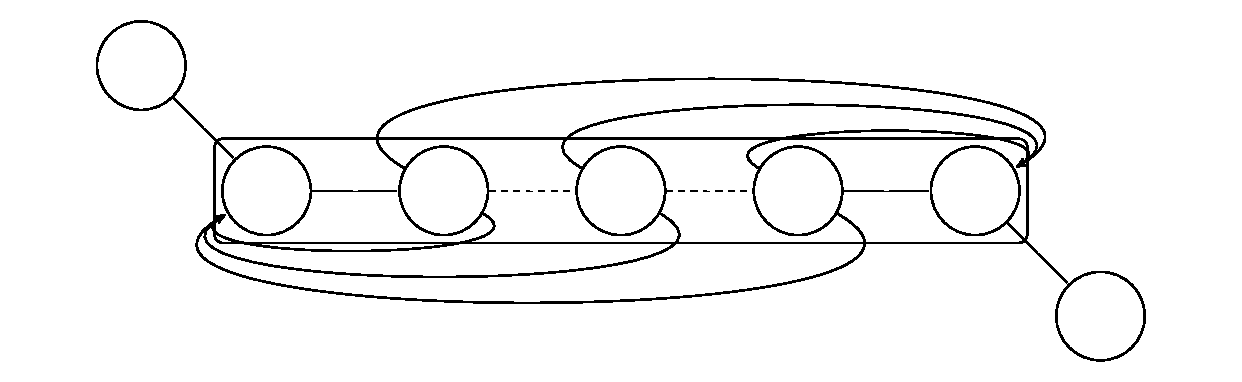
\includegraphics[scale=.7]{Imagenes/N4.pdf}
\caption{Movimientos de la vecindad N4}
\end{figure}


\item N5 \cite{EugeniuszNowicki2003} Consiste en intercambiar solo las operaciones adyacentes a la final o inicial de un bloque crítico.  
\begin{figure}[H]
\centering
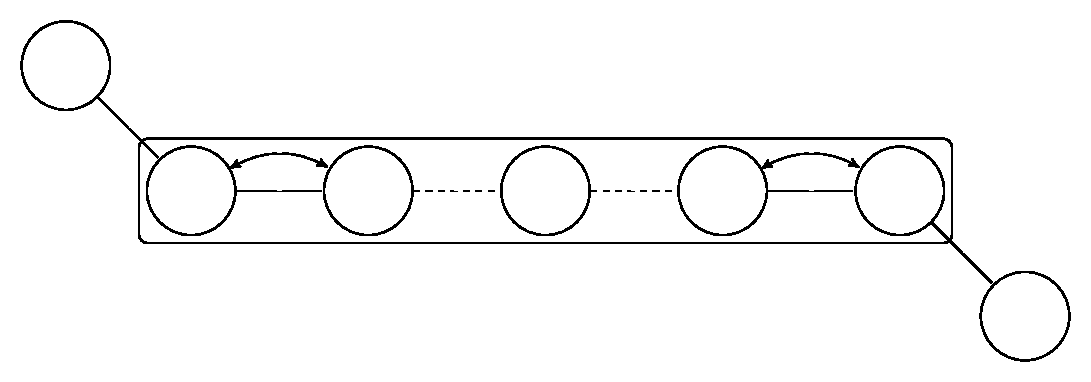
\includegraphics[scale=.7]{Imagenes/N5.pdf}
\caption{Movimientos de la vecindad N5}
\end{figure}

\item N6 \cite{Balas1998} Los autores utilizan varios teoremas para identificar pares $(u,v)$ de operaciones dentro de un bloque crítico que puedan llevar a mejorar la solución y a su vez identificar si se tiene que mover a $u$ justo después de $v$(forward) o bien a $v$ justo antes de $u$ (backward).
\begin{figure}[H]
\centering
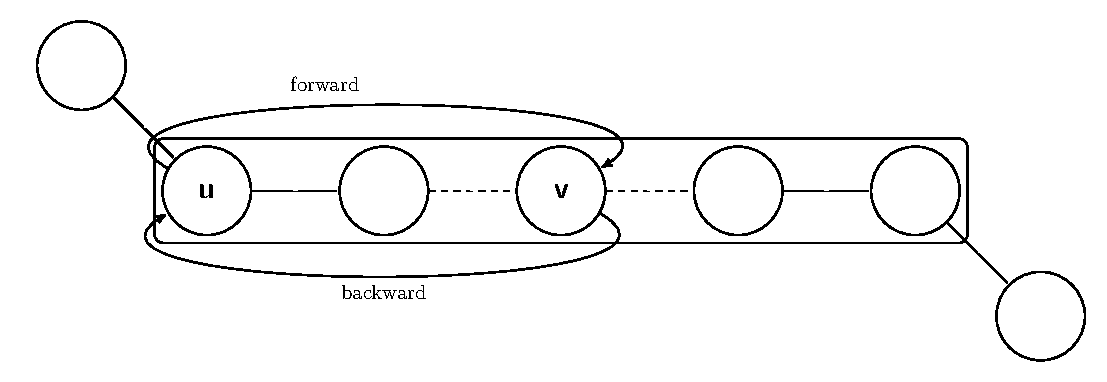
\includegraphics[scale=.7]{Imagenes/N6.pdf}
\caption{Los dos tipos de movimientos para un par $(u,v)$}
\end{figure}

\item N7 \cite{Zhang2007} Esta vecindad se plantea como una extensión de la N6 en la cual se toma la idea de los movimientos entre pares de operaciones de un bloque crítico. Los autores toman en cuenta todos los cambios posibles entre el inicio o fin del bloque crítico con todas las operaciones internas.

\begin{figure}[H]
\centering
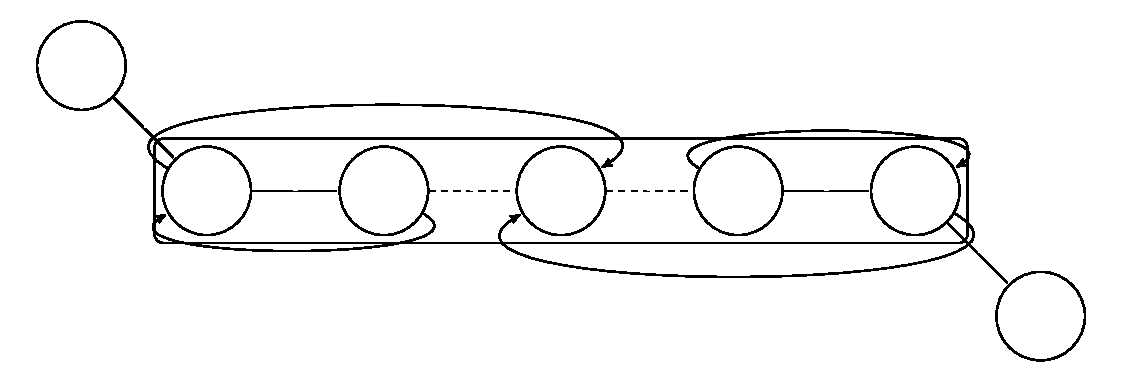
\includegraphics[scale=.7]{Imagenes/N7.pdf}
\caption{Movimientos de la vecindad N7}
\end{figure}
\end{itemize}

